\section{The Biased KDE Approach and Conservative Reformulation}
\label{ch:biasedkde}

Chapter~3 closed on a measured verdict: the unbiased reformulation is an
accuracy method, not a safety method, and its certificate fails almost
as often as not. This chapter converts the verdict into a construction.
The repair is not a patch applied after estimation but a redesign of the
estimator itself, due to \citet{keil2020,keil2021}: choose the kernel so
that smoothing and conservatism become the same act, exactly the
property previewed in Chapter~2's kernel figure and now developed in
full. The chapter states the requirement the unbiased estimator fails
(\cref{sec:notsafe}), formalizes the domination condition that defines a
biased kernel (\cref{sec:biasing}), examines the three kernels that
matter in practice and the precise sense in which each satisfies or
approximates the condition (\cref{sec:biasedkernels}), assembles the
conservative reformulation pipeline and prices its conservatism on a
known-truth problem (\cref{sec:biasedreform}), and then extends the
framework to joint chance constraints through three competing routes
(\cref{sec:jointthree}), of which the scalar violation statistic with
log-sum-exp smoothing (\cref{sec:lse}) is this thesis's recommended
extension and one of its main implementation contributions. The chapter
closes with the bandwidth-continuation strategy that makes the whole
construction solvable in practice (\cref{sec:continuation}).

\subsection{Why Smoothing Alone Is Not Safe}
\label{sec:notsafe}

The limitation must be located precisely before it can be addressed,
because it does not lie where one might first look. The unbiased
estimator of Chapter~3 is consistent, its bandwidth theory is classical,
and its certificate concentrates near the target; none of its
statistical properties is at fault. The limitation is directional. A symmetric kernel's
integrated form crosses the indicator at the constraint boundary, so
each sample's contribution to $\hat{p}_h(x)$ errs toward optimism for
violating residuals and toward pessimism for safe ones, and nothing in
the construction controls which effect dominates at the decision the
optimizer actually returns. The optimizer, moreover, is not a neutral
party: it systematically favors the cheapest certified decision, which
tends to be a decision at which optimistic error contributed to the
certificate being granted. Chapter~3 measured the result at
$39\%$ certificate failure.

For engineering and safety-critical applications this behavior is
problematic, and the requirement that replaces it can be stated in one
line. What is
needed is an estimator that never credits a violating sample: a
surrogate $\hat{p}_h^{\,b}$ whose every per-sample contribution is
bounded by the indicator it replaces, so that
$\E[\hat{p}_h^{\,b}(x)] \leq \Prob(g(x,\xi) \leq 0)$ at every decision,
and any solution certified by the surrogate satisfies the true chance
constraint in expectation. Equivalently, in the violation form of
Chapter~2, the surrogate violation estimate must dominate the true
violation probability from above. The estimator may still err, but the construction ensures that its
errors no longer point in the unsafe direction.

\subsection{The Biasing Construction}
\label{sec:biasing}

The construction of \citet{keil2020} unifies two half-solutions, each
inadequate alone. The first replaces the violation indicator
$\ind\{t > 0\}$ with any function $w(t) \geq \ind\{t > 0\}$: averaging
$w$ over samples always upper-bounds the violation probability, but $w$
need not be bounded by one, so the average is not a valid probability
and distorts the optimization. The second is the standard KDE surrogate
of Chapter~3, a valid CDF bounded in $[0,1]$ that violates the
domination requirement. The biased kernel is the object that holds both
properties at once. A kernel $K$ with integrated form $F_K$ and bias
term $b(h) \geq 0$ satisfies the \emph{domination condition} when its
safe-side surrogate is bounded by the indicator,
\begin{equation}
  F_K\!\left(\frac{-\,t - b(h)}{h}\right) \;\leq\; \ind\{t \leq 0\}
  \qquad \text{for all } t \in \R \text{ and } h > 0 ,
  \label{eq:domination}
\end{equation}
equivalently, when the complementary violation surrogate dominates
$\ind\{t > 0\}$ from above for every residual. Condition
\cref{eq:domination} asks for exactly one thing beyond Chapter~3: the
surrogate must vanish on the entire violating half-line $t > 0$, which
the bias $b(h)$ accomplishes by shifting the kernel's mass to the safe
side of the boundary.

The conservative estimator and constraint follow immediately. Averaging
the dominated surrogate over the residual samples of Chapter~3 gives
\begin{equation}
  \hat{p}_h^{\,b}(x)
  \;=\; \frac{1}{N}\sum_{j=1}^{N}
  F_K\!\left(\frac{-\,g(x,\xi_j) - b(h)}{h}\right),
  \qquad
  \hat{p}_h^{\,b}(x) \;\geq\; 1-\varepsilon ,
  \label{eq:biasedcc}
\end{equation}
and the safety statement is now a provable property rather than an
empirical observation: since each
term of \cref{eq:biasedcc} is bounded by the corresponding indicator,
$\E[\hat{p}_h^{\,b}(x)] \leq \Prob(g(x,\xi) \leq 0)$ pointwise, so any
decision satisfying the biased constraint satisfies the true chance
constraint in expectation, with only sampling fluctuation, vanishing as
$N$ grows, standing between the certificate and the guarantee.
\Cref{fig:domination}(a) draws the construction: the unbiased surrogate
crosses the indicator and grants credit to violating samples (the
optimism Chapter~3 measured), while the biased surrogate sits entirely
beneath it, discounting boundary samples and crediting violations
nothing at all. Smoothness has not been spent to buy safety; the biased
surrogate is exactly as differentiable as the unbiased one, and every
formula of Chapter~3, the closed-form constraint, the analytic gradient,
the $N$-independent program size, survives with $-g(x,\xi_j)$ replaced
by $-g(x,\xi_j) - b(h)$. In the language of the two error sources
separated in Chapter~3, the bias acts on the smoothing error alone: the
sampling error remains random and vanishes with $N$, while the
smoothing error is now signed toward safety rather than merely made
small.

\begin{figure}[t]
  \centering
  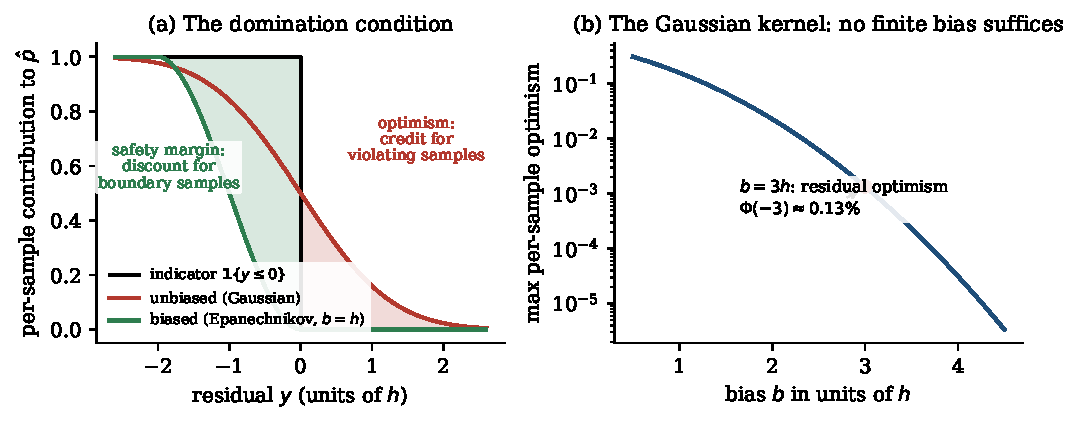
\includegraphics[width=\textwidth]{kap04/figures/fig_domination.pdf}
  \caption{The biasing construction. (a) Per-sample contributions to the
  probability estimate, in units of the bandwidth. The unbiased Gaussian
  surrogate crosses the indicator and credits violating residuals
  (shaded right), the optimism measured in Chapter~3; the biased
  Epanechnikov surrogate with $b = h$ sits entirely beneath the
  indicator, so every per-sample error points to the safe side (shaded
  left). (b) Why the Gaussian kernel cannot be made exactly safe: its
  maximal per-sample optimism $\Phi(-b/h)$ is positive for every finite
  bias, decaying but never vanishing; $b = 3h$ leaves a residual
  optimism of $0.13\%$ per sample.}
  \label{fig:domination}
\end{figure}

\subsection{Specific Biased Kernels}
\label{sec:biasedkernels}

Condition \cref{eq:domination} is a constraint on kernel tails, and the
three kernels of Chapter~2 meet it in three instructively different
ways. The \emph{split-Bernstein kernel}, a piecewise-polynomial
construction originating in approximation theory and adapted to chance
constraints by \citet{keil2021}, satisfies the domination condition
exactly for appropriate parameter choices: its compact, one-sided
structure is designed around \cref{eq:domination} rather than retrofitted
to it, and its integrated form is smooth and available in closed form.
It is the reference kernel whenever the strict guarantee is the
priority. The \emph{Epanechnikov kernel with bias} starts from the
AMISE-optimal kernel of Chapter~2 and exploits its compact support: with
$b(h) = h$, the shifted surrogate vanishes identically on the violating
half-line, so \cref{eq:domination} holds exactly, and in the lunar
landing experiments of \citet{keil2021} this kernel achieves the lowest
average optimal cost among the biased family, the statistical efficiency
of Chapter~2 carrying over into the optimization.

The \emph{Gaussian kernel} is the cautionary member, and its limitation
here is structural rather than incidental: because its tails are
strictly positive everywhere, no finite bias can make the surrogate
vanish for $t > 0$, so the Gaussian cannot satisfy \cref{eq:domination}
exactly \citep{keil2021}. \Cref{fig:domination}(b) quantifies the gap. The
maximal per-sample optimism after biasing is $\Phi(-b/h)$, positive for
every finite $b$; the practical compromise $b \approx 3h$ caps it at
$\Phi(-3) \approx 0.13\%$, covering $99.87\%$ of the tail and rendering
the kernel \emph{approximately} conservative. The Gaussian's
compensating virtues are real, infinite smoothness and the fastest
solver runtimes in the family, and the resulting division of labor is
the one this thesis adopts: Gaussian kernels where speed and smoothness
dominate, exact biased kernels where the guarantee does, and the
continuation strategy of \cref{sec:continuation} to move between them
within a single solve.

\subsection{Stochastic Optimization Reformulated via Biased KDE}
\label{sec:biasedreform}

The full conservative pipeline assembles the chapters of Part~3 into
five steps, stated once here as the procedure the experimental chapters
implement. First, generate $N$ samples $\xi_1,\dots,\xi_N$ by
simulation, Markov chain Monte Carlo, or historical data, exactly as in
Chapter~2. Second, for each candidate decision $x$, form the residuals
$y_j(x) = g(x,\xi_j)$ of Chapter~3. Third, evaluate the biased
constraint function $\hat{p}_h^{\,b}(x)$ of \cref{eq:biasedcc} with a
kernel and bias from \cref{sec:biasedkernels}. Fourth, enforce
$\hat{p}_h^{\,b}(x) \geq 1-\varepsilon$. Fifth, solve the resulting
deterministic nonlinear program with the analytic derivatives that the
construction provides. The program retains every structural property of
Chapter~3: one smooth inequality, size independent of $N$, gradients by
the chain rule.

What the bias changes is the trade, and \cref{fig:safetycost} prices it
on the dispatch problem where the truth is computable. The comparison is
the one promised in Chapter~3's closing: the unbiased reformulation is
smooth and less conservative but carries no finite-sample safety, while
the biased reformulation is slightly more conservative and carries it.
The numbers make the asymmetry of the trade explicit. Across sample
sizes, the unbiased certificate fails in roughly $34$ to $43\%$ of
trials and does not improve with data, because its error is directional,
not statistical; the biased certificate fails in $14\%$ of trials at
$N = 50$, falls to $5\%$ by $N = 200$, and is below $1\%$ from
$N = 500$, the residual failures being pure sampling fluctuation around
a safe-side mean. The premium paid for this is $2.6$ to $4\%$ of
objective value, shrinking as $N$ grows. This exchange is familiar from reliability engineering: a bounded and
vanishing cost in return for removing a class of certificate failures.
The unbiased method answers the question \emph{what is the
probability}; the biased method answers the question the application
typically asks, \emph{can this decision be trusted}.

\begin{figure}[t]
  \centering
  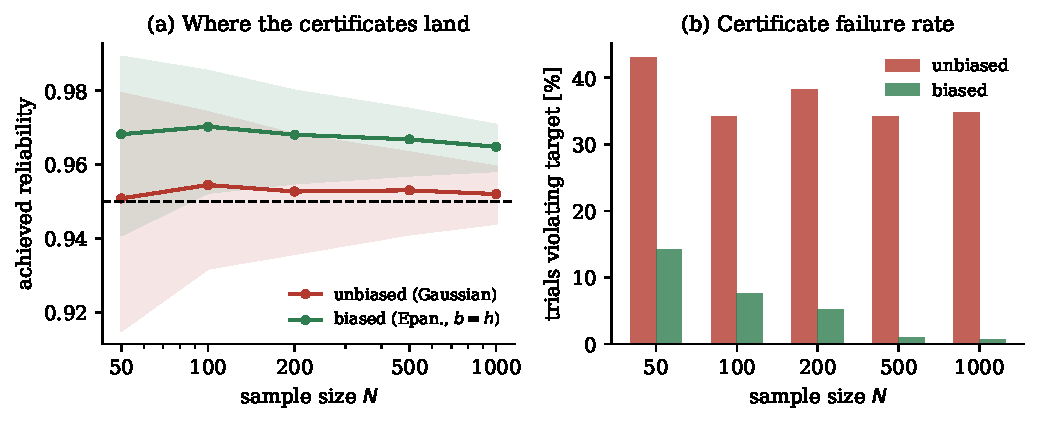
\includegraphics[width=\textwidth]{kap04/figures/fig_safetycost.pdf}
  \caption{The price and the purchase of conservatism, on the dispatch
  problem ($\varepsilon = 0.05$, $800$ trials per sample size, bands are
  $10$th-to-$90$th percentiles). (a) The unbiased certificate straddles
  the target from below on a large fraction of trials at every $N$; the
  biased certificate (Epanechnikov, $b = h$) lands above it by a margin
  that shrinks as the estimator sharpens. (b) Certificate failure rates:
  the unbiased rate is structural and does not improve with data; the
  biased rate is sampling fluctuation and collapses, falling below
  $1\%$ from $N = 500$. The average objective premium paid for safety is
  $2.6$ to $4\%$, decreasing in $N$.}
  \label{fig:safetycost}
\end{figure}

\subsection{Joint Chance Constraints: Three Approaches}
\label{sec:jointthree}

Everything so far concerns a scalar residual. The joint constraint of
Chapters~1 through~3,
$\Prob(g_r(x,\xi) \leq 0,\, r = 1,\dots,m) \geq 1-\varepsilon$, asks
about $m$ requirements at once, and the biased framework extends to it
along three routes whose trade-offs this subsection fixes, because the
choice among them is a design decision the experimental chapters revisit.

\emph{Approach A: Boole's inequality with risk allocation.} The union
bound $\Prob(\bigcup_r \{g_r > 0\}) \leq \sum_r \Prob(g_r > 0)$ yields a
sufficient condition: enforce each component at level $\varepsilon_r$
with $\sum_r \varepsilon_r \leq \varepsilon$, applying the
one-dimensional biased KDE of \cref{sec:biasedreform} to each residual
separately \citep{prekopa1995,keil2021}. The route is simple, fully
tractable, and conservative twice over, once through the bias and once
through the union bound; its conservatism grows with $m$ and is most
costly exactly when the component violations are strongly correlated,
the case the union bound prices worst.

\emph{Approach B: multivariate KDE.} Estimate the joint density of the
residual vector $(g_1(x,\xi),\dots,g_m(x,\xi))$ with a multivariate
kernel and bandwidth matrix $H$, and integrate over the safe orthant
$(-\infty,0]^m$ \citep{wu2021,wu2023}. The route is exact in the sense
that no decomposition is imposed, but it reintroduces precisely the
difficulty the residual-space construction was designed to avoid: the
curse of dimensionality of Chapter~2 now acts in the constraint
dimension $m$,
and the sample sizes it demands grow exponentially.

\emph{Approach C: the scalar violation statistic.} The recommended
extension of this thesis collapses the joint constraint exactly. For
positive weights $w_r$, define
\begin{equation}
  s(x,\xi) \;=\; \max_{r = 1,\dots,m} \, w_r\, g_r(x,\xi) .
  \label{eq:scalarstat}
\end{equation}
The reduction is an identity, not a bound: all components are
nonpositive precisely when their weighted maximum is, so
\begin{equation}
  \Prob\bigl(g_r(x,\xi) \leq 0,\; r = 1,\dots,m\bigr)
  \;=\; \Prob\bigl(s(x,\xi) \leq 0\bigr) ,
  \label{eq:exactreduction}
\end{equation}
and the joint chance constraint is a scalar chance constraint on
$s$. A one-dimensional biased KDE suffices; no Boole decomposition, no
multivariate estimation, no curse of dimensionality. The constraint map
itself has once again performed the dimension reduction, now in $m$ as
well as in $d$. The single catch is the one Chapter~2 anticipated: the
max in \cref{eq:scalarstat} is nonsmooth, and a nonsmooth residual would
re-break exactly the differentiability that Chapter~3 worked to
establish. Removing that catch is the purpose of the next subsection.

\subsection{Log-Sum-Exp Smoothing of the Scalar Violation Statistic}
\label{sec:lse}

The max is smoothed by the log-sum-exp surrogate with temperature
$\tau > 0$,
\begin{equation}
  s_\tau(x,\xi)
  \;=\; \tau \log\!\left(\sum_{r=1}^{m}
  \exp\!\left(\frac{w_r\, g_r(x,\xi)}{\tau}\right)\right),
  \label{eq:lse}
\end{equation}
which satisfies the two-sided bound
\begin{equation}
  \max_r\, w_r\, g_r(x,\xi)
  \;\leq\; s_\tau(x,\xi)
  \;\leq\; \max_r\, w_r\, g_r(x,\xi) + \tau \log m ,
  \label{eq:lsebounds}
\end{equation}
\citep{boyd2004}. The direction of the bound is the key property of the construction,
and it should be read in the spirit of
\cref{eq:domination}: the surrogate dominates the true statistic, so
enforcing $\Prob(s_\tau \leq 0) \geq 1-\varepsilon$ \emph{implies} the
true joint constraint, and the smoothing error, like the kernel bias, is
conservative by construction. The temperature plays for the max exactly
the role the bandwidth plays for the indicator: a smoothing parameter
whose cost is a controlled, safe-side margin of at most
$\tau \log m$. \Cref{fig:lse}(a) shows the geometry on a two-constraint
slice, $s_\tau$ riding above the kink and collapsing onto it as $\tau$
shrinks.

The gradient completes the smoothness argument. Differentiating
\cref{eq:lse} gives
\begin{equation}
  \nabla_x\, s_\tau(x,\xi)
  \;=\; \sum_{r=1}^{m} \pi_r(x,\xi)\, w_r\, \nabla_x\, g_r(x,\xi),
  \qquad
  \pi_r \;=\;
  \frac{\exp\bigl(w_r g_r / \tau\bigr)}
       {\sum_{q} \exp\bigl(w_q g_q / \tau\bigr)} ,
  \label{eq:lsegrad}
\end{equation}
a softmax-weighted blend of the component gradients, smooth in $x$ and
analytically computable. \Cref{fig:lse}(b) shows the weights handing
influence from one constraint to the other across the switching point,
continuously, where the raw max would switch abruptly and
nondifferentiably. Composing the pieces yields the full biased-KDE
reformulation for joint constraints,
\begin{equation}
  \frac{1}{N}\sum_{j=1}^{N}
  F_K\!\left(\frac{-\,s_\tau(x,\xi_j) - b(h)}{h}\right)
  \;\geq\; 1-\varepsilon ,
  \label{eq:jointreform}
\end{equation}
and \cref{eq:jointreform} is one of this thesis's main implementation
contributions, a claim supported by what the formulation absorbs: a
joint,
non-Gaussian, possibly high-dimensional chance constraint has been
reduced to a single smooth one-dimensional deterministic inequality,
with two stacked approximation layers, kernel bias and log-sum-exp
temperature, both of which err on the safe side by construction. The
interaction of those two layers, how conservatism compounds across
$h$ and $\tau$ and how the budget should be split between them, is a
genuinely open question, and it is studied experimentally as research
question RQ4 in Part~4.

\begin{figure}[t]
  \centering
  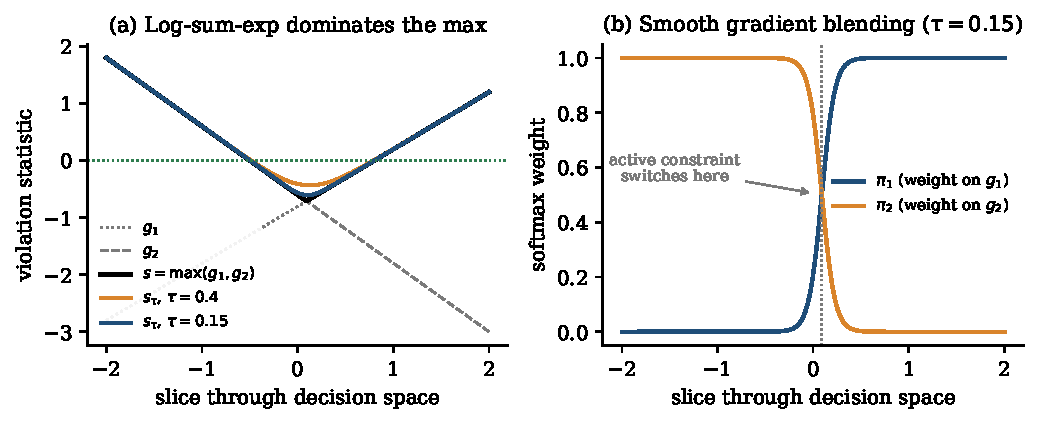
\includegraphics[width=\textwidth]{kap04/figures/fig_lse.pdf}
  \caption{Log-sum-exp smoothing of the scalar violation statistic on a
  two-constraint slice. (a) The surrogate $s_\tau$ dominates
  $s = \max(g_1, g_2)$ everywhere, with gap at most $\tau \log m$
  concentrated at the kink; as $\tau$ shrinks the surrogate collapses
  onto the max, so the smoothing error is a tunable, safe-side margin.
  (b) The softmax weights of the gradient formula hand influence from
  one constraint to the other continuously across the switching point,
  giving the solver a smooth blend where the raw max would give a
  nondifferentiable jump.}
  \label{fig:lse}
\end{figure}

\subsection{Bandwidth Continuation and Kernel Switching}
\label{sec:continuation}

The constructions of this chapter create a practical tension that one
further idea resolves. Small bandwidths and exactly-safe kernels are
where the guarantees live, but they are also where the optimization is
hardest: a sharply smoothed constraint approaches the staircase of
Chapter~2, and a solver started cold against it inherits a rugged,
nearly nonsmooth landscape. The warm-start strategy of
\citet{keil2021warm} converts this tension into a schedule.
\Cref{fig:continuation} draws it. Begin with a large bandwidth, where
the constraint is heavily smoothed, the landscape benign, and the
Gaussian kernel's speed available; solve, and pass the solution forward
as the initial point for a smaller bandwidth; repeat, increasing the
sample size as the bandwidth shrinks so that statistical resolution
keeps pace with geometric resolution; and near convergence, switch from
the Gaussian to an exactly-safe kernel, the split-Bernstein, so that the
final certificate carries the strict guarantee of
\cref{sec:biasedkernels} rather than the $99.87\%$ approximation.

\begin{figure}[t]
  \centering
  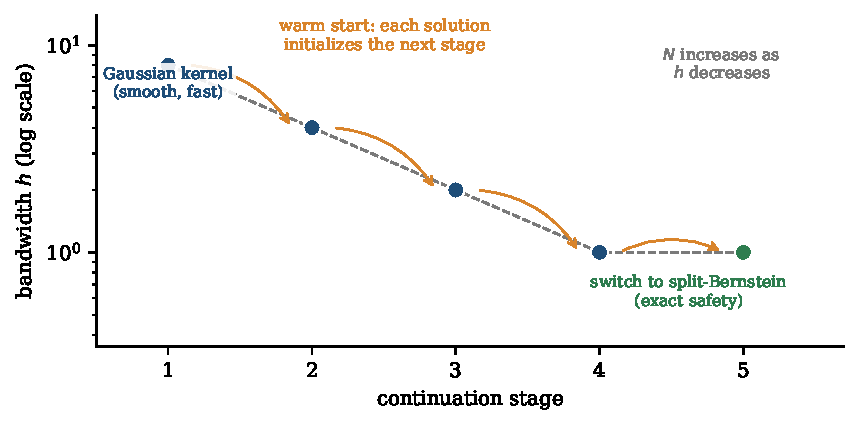
\includegraphics[width=0.82\textwidth]{kap04/figures/fig_continuation.pdf}
  \caption{The bandwidth-continuation and kernel-switching schedule of
  \citet{keil2021warm}. Early stages use a large bandwidth and the fast
  Gaussian kernel, producing a benign landscape and a cheap solution;
  each stage's solution warm-starts the next as the bandwidth shrinks
  and the sample size grows; the final stage switches to the
  split-Bernstein kernel so that the converged certificate carries the
  exact domination guarantee. The homotopy stabilizes the solver and
  avoids the numerical difficulty of attacking a small-bandwidth,
  nearly nonsmooth constraint from a cold start.}
  \label{fig:continuation}
\end{figure}

The schedule is a homotopy in the proper sense: a continuous deformation
from an easy problem to the target problem along which the solution is
tracked rather than rediscovered, and its effect in the experiments of
\citet{keil2021warm} is precisely the one homotopies exist to deliver,
stabilized convergence and substantially reduced solve times relative to
cold starts at the final bandwidth. With it, Part~3 is complete as a
method: a conservative, smooth, one-dimensional, $N$-independent
reformulation for individual and joint chance constraints, equipped with
a practical solution strategy. What the method still lacks is a formal
guarantee that its answers approximate \emph{the true problem}, in the
sense that as data accumulates the reformulated solutions converge to
the true ones. Supplying that license is the
convergence theory of \citet{schuster2025}, and connecting it to the
constructions of this chapter is the work the next chapter takes up.
